\section{Wyliczanie rankingu dokumentów}

Wyszukiwanie dokumentów jest akcją, która zostaje zapoczątkowana przez użytkownika, poprzez wpisanie odpowiedniego zapytania. Zapytanie to jest w postaci słowa przesyłane jest na serwer, razem z parametrami (wagami) wpływającymi na końcowy ranking dokumentu.

\begin{figure}[htb]
\centering
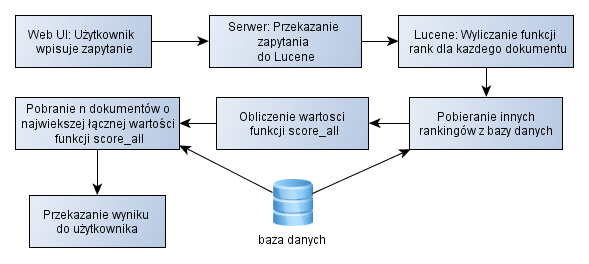
\includegraphics[width=\textwidth]{search.png}
\caption{Proces wyszukiwania w postaci schematu}
\label{fig:wyszukiwanie}
\end{figure}

Pierwszym krokiem otrzymania wyszukiwanych dokumentów jest przekazanie zapytania do frameworku Lucene. W tym systemie zapytanie jest czyszczone i zamieniane na odpowiednie tokeny. Następnie tworzony jest zbiór dokumentów zawierających poszukiwane słowa. 

\begin{figure}[htb]
\centering
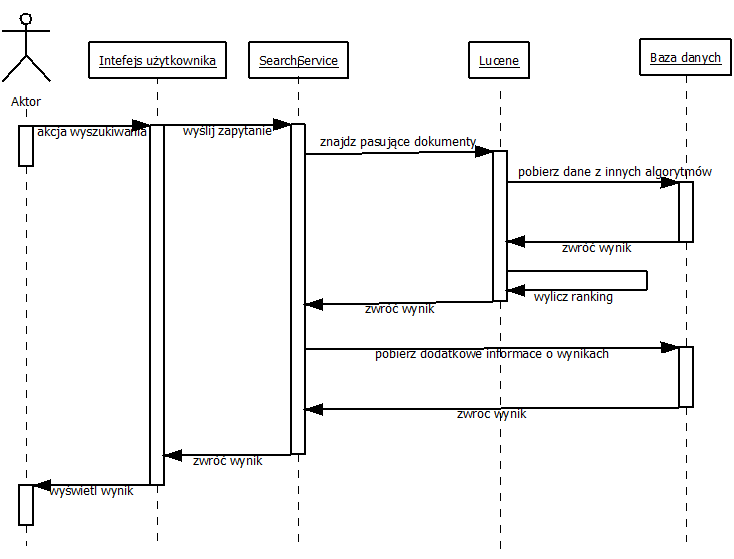
\includegraphics[width=\textwidth]{diagram_przebiegu_wyszukiwania.png}
\caption{Diagram przebiegu wyszukiwania}
\label{fig:wyszukiwanie_diagram_seq}
\end{figure}

Każdy dokument z tego zbioru ma przydzieloną wartość rankingu Lucene, wyznaczoną przy użyciu funkcji TF-IDF. Jest to pierwszy z czynników wpływających na ostateczny wynik klasyfikacji dokumentu. Dla każdego otrzymanego dokumentu, z bazy danych pobierane są informacje o ich rankingach uzyskanych za pomocą algorytmów  AdaptedPageRank, SocialPageRank i danych otrzymanych z innych serwisów społecznościowych (Twitter, Facebook, Digg). 

Każdy z cząstkowych rankingów wpływających na ostateczny wynik ma przydzieloną wagę. Waga ta może zostać zmieniona z poziomu interfejsu użytkownika. Ranking dokumentu wyliczany jest według wzoru \ref{eq:final_rank}.




